% !TEX root = main.tex
\chapter{Objectives}\label{sec:methods} %and goals of ReviewerNet}

The aim of ReviewerNet is to facilitate the reviewer selection process in the academic domain. While designing ReviewerNet, we took into account the characteristics of the \emph{users}, the users' \emph{tasks}, and the \emph{data} the users are working with \cite{MiAi14}. 

The \emph{users} of ReviewerNet are researchers, and in particular those playing the role of journal editors, associate editors, and members of IPCs of big conferences, in any field of research. Their \emph{task} is searching for reviewers for a submitted paper: this involves searching the literature for key papers and authors in the field; evaluating the candidates' research interests and their evolution over time; and assessing the candidates' conflict of interest with respect to the submitting authors and other reviewers. ReviewerNet supports all these subtasks, by visualizing the literature related with a topic, the career of relevant researchers in the field, and the relationships among researchers. 

The data pertain to three types of entities: \emph{papers}, \emph{researchers}, and \emph{citations}. The data attributes are both quantitative and qualitative, and the time dimension is central. 

In ReviewerNet, the attributes of a paper which are visualized are its \emph{citation count} -- the number of papers citing it -- as well as standard \emph{bibliographic attributes} -- title, authors, publication year, venue. Papers are related through \emph{direct citations}. 

Researchers have two attributes in ReviewerNet: relevance and conflict of interest. We define a researcher's \emph{relevance} as a reviewer according to the authorship of relevant papers. The concept of relevance can be tuned according to the user needs (e.g., looking for highly-specialized reviewers, as opposed to generalists). The second attribute of researchers is their \emph{conflict of interest}, with either the submitting authors or other reviewers. We model the conflict of interest after \emph{co-authorship} relations: two researchers have a conflict of interest if they have papers in common. We let the degree of conflict, and hence the availability as a reviewer, be modulated according to the number of papers in common, and the years passed since the last co-authored paper, again according to the user intent. 

The following section details the notation used in the rest of the paper, and the formal definition of paper and researcher attributes. 

\section{Notation}

Let $\mathcal{P}$ denote the set of papers in a reference dataset, %, with cardinality $\vert \mathcal{P} \vert$, 
and let $\mathcal{P}_{V} \subseteq \mathcal{P}$ be the set of papers relevant to a submission. %, with $\mathcal{P}_{V} \subseteq \mathcal{P}$. The set $\mathcal{P}_{V}$ of relevant papers 
$\mathcal{P}_{V}$ is built by the users starting from a small number of seed papers of their choice (cf. Section \ref{sec:demoPN}).%, through the graph expansion functionalities offered by the Paper Network visualization.   

A paper $p \in \mathcal{P}_{V}$ is marked as \emph{selected}, if it is considered as a key paper by the user; we denote by $\mathcal{P}_{S}$ the set of selected papers, with $\mathcal{P}_{S} \subseteq \mathcal{P}_{V} \subseteq \mathcal{P}$. 

If $\mathcal{C}(p)$ is the set of papers citing $p$, the \emph{citation count} $c(p)$ is its cardinality: $c(p) = \vert \mathcal{C}(p) \vert$.

Let $\mathcal{A}(p)$ be the set of authors of a given paper $p$, and $\mathcal{R}$ the set of authors of papers in $\mathcal{P}$. 
%, and $\mathcal{R}_{V}$ be the set of authors of papers in $\mathcal{P}_{V}$: $\mathcal{R}_{V} = \{r \in \mathcal{R} \ s.t. \ \exists \ p \in \mathcal{P}_V : r \in \mathcal{A}(p)\}$. 
Then, the set $\mathcal{R}_C \subseteq \mathcal{R}$ of \emph{candidate reviewers} is given by the set of researchers who authored a selected paper: $$\mathcal{R}_{C} = \{r \in \mathcal{R} \ s.t. \ \exists \ p \in \mathcal{P}_S : r \in \mathcal{A}(p)\}$$ %It holds that $\mathcal{R}_C \subseteq \mathcal{R}_{V} \subseteq \mathcal{R}$.  
%
For a candidate reviewer $r$, let $\mathcal{P}_{S}|_{r}$ be the set of papers in $\mathcal{P}_{S}$ authored by $r$. Then, the \emph{relevance score} $s(r)$ of the candidate reviewer $r$ is defined as a weighted sum of the number of selected and non-selected papers in $\mathcal{P}_V$ authored by $r$: $$s(r) = \alpha \vert \mathcal{P}_{S}|_{r} \vert + \beta \vert \{\mathcal{P}_{V} - \mathcal{P}_{S}\}|_{r}\vert$$ with $\alpha$ and $\beta$ real-valued coefficients summing up to one. We set $\alpha = 0.7$ and $\beta = 0.3$ as default parameters. The set of candidate reviewers will be visualized in the Researcher Timeline in order of their relevance; relevance will also define the dimension of nodes in the Researcher Network.

Finally, $\mathcal{CA}(r)$ denotes the set of co-authors of a researcher $r$, or, in other words, the set of researchers who have a conflict with him/her. 


\chapter{User interface}
\label{sec:userinterface}

There are four regions in the user interface, described below and shown in Figure~\ref{fig:interface}. Each region is resizable in height. The visual composition helps the user to gain different perspectives on the problem at hand, within a single visualization. \\


\noindent{\bf The Paper Network:} 
The Paper Network (PN), at the bottom-left hand side of the screen, is a graph visualization of the literature relevant to a submission topic. The nodes represent papers in $\mathcal{P}_{V}$, while the arcs represent in- and out-citation relations between them. The horizontal dimension represents time, as papers are ordered according to their publication year. A force-directed graph drawing algorithm determines the layout in the vertical direction. The Paper Network is built interactively by the user. 
\\

\noindent{\bf The Researcher Timeline:} 
The Researcher Timeline (RT), at the upper-left side of the screen, is a visualization of the academic career of researchers, through lines and bars. Each line represents a candidate reviewer $r$ in $\mathcal{R}_{C}$, that is, the author of a selected paper in $\mathcal{P}_{S}$. The dots over the line represent the set $\mathcal{P}|_{r}$ of papers authored by $r$ in the reference database $\mathcal{P}$. The Researcher Timeline is constructed and updated automatically by ReviewerNet while the user builds and refines the Paper Network.  \\

\noindent{\bf The Researcher Network:} 
The Researcher Network (RN), at the upper-right hand side of the screen, is a graph visualization of the co-authorship relations. The nodes are the researchers in $\mathcal{R}_V$ along with their collaborators in $\mathcal{R}$. The arcs connect authors who have publications in common: for each node representing a researcher $r$, the node degree is the cardinality $\vert \mathcal{CA}(r) \vert$. A force-directed graph drawing algorithm determines the graph layout. As with the Researcher Timeline, the Researcher Network is built automatically by ReviewerNet while the user builds the Paper Network.  \\

\noindent{\bf The Control Panel:} 
The Control Panel (CP), at the bottom-right hand side of the screen, allows the user to input and manage the names of submitting authors, the names of selected reviewers, and the titles of key papers. The CP area also displays information about papers, upon request. The DBLP icon beside reviewers' names and paper titles links to their respective DBLP page. Moreover, the CP includes parameters boxes and checkboxes to fine-tune the visualization (cf. Section \ref{subsec:parameters}). Finally, the CP enables the user to download the list of selected reviewers, along with substitute reviewers suggested by ReviewerNet.  

\begin{figure*}[!pt]
\centering
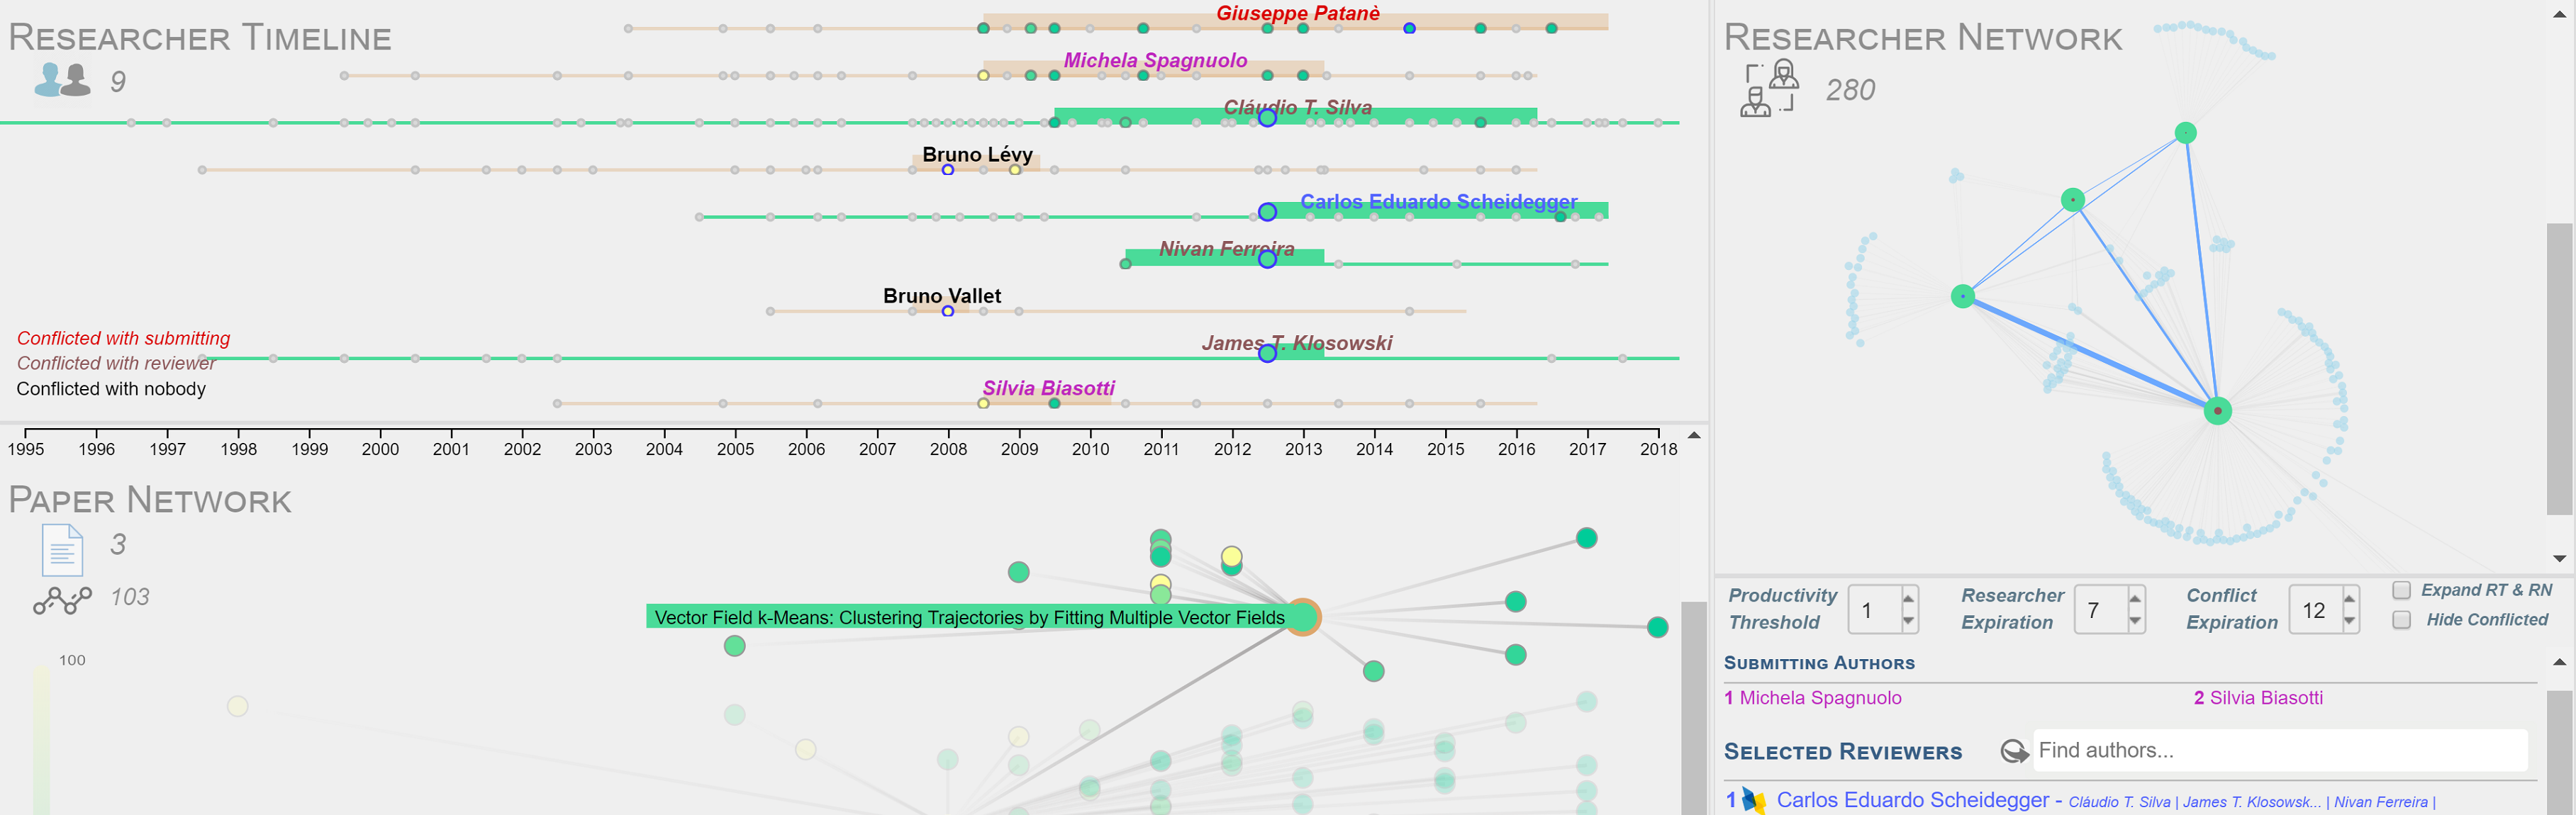
\includegraphics[width=\textwidth]{images/paperhovering_crop.png}
\caption{When hovering over an entity representing a paper, the authors of that paper are highlighted in the other views.}
\label{fig:paperhovering}
\end{figure*}


\section{Visual consistency}
\label{subsec:visualvar}

Visual cues include the colour, size, boundary, and style of visual elements representing papers, researchers and their relations across the different views.  \\

%\noindent{\bf Visual cues for papers}
\noindent{\bf Visual cues for papers:} 
For a paper $p \in \mathcal{P}_{V}$, the color corresponds to the citation count $c(p)$, from yellow (few citations) to green (many citations). This colormap applies to both nodes in the PN and dots in the RT. Dots corresponding to papers in $\mathcal{P} - \mathcal{P}_V$ (papers in the reference database, but not included the PN) are marked as grey. 

Selected papers in $\mathcal{P}_S$ are circled in blue, both in the PN and the RT.  Arcs are blue in the RN when the co-authored papers include a selected paper.  \\

\noindent{\bf Visual cues for researchers:} 
For researchers in the RT, the name coloring emphasizes the distinction between roles: submitting authors (marked as purple), their co-authors (red), selected reviewers (blue), their co-authors (brown), and non-conflicting, candidate reviewers (black). The nodes in the RN corresponding to researchers in the RT follow the same rule, whereas nodes representing their co-authors in $\mathcal{R}$ are light blue.   

For researchers in the RT, the font style of names further helps to tell apart conflicting researchers (italic) from non-conflicting candidate reviewers (normal). The same colour/font rules apply to the names suggested in the selected reviewers' drop-down menu in the CP.

The researchers in the RT are ordered vertically according to their relevance score $r(s)$. The same score is rendered in the RN through the dimension of nodes.  \\


\begin{figure*}
\centering
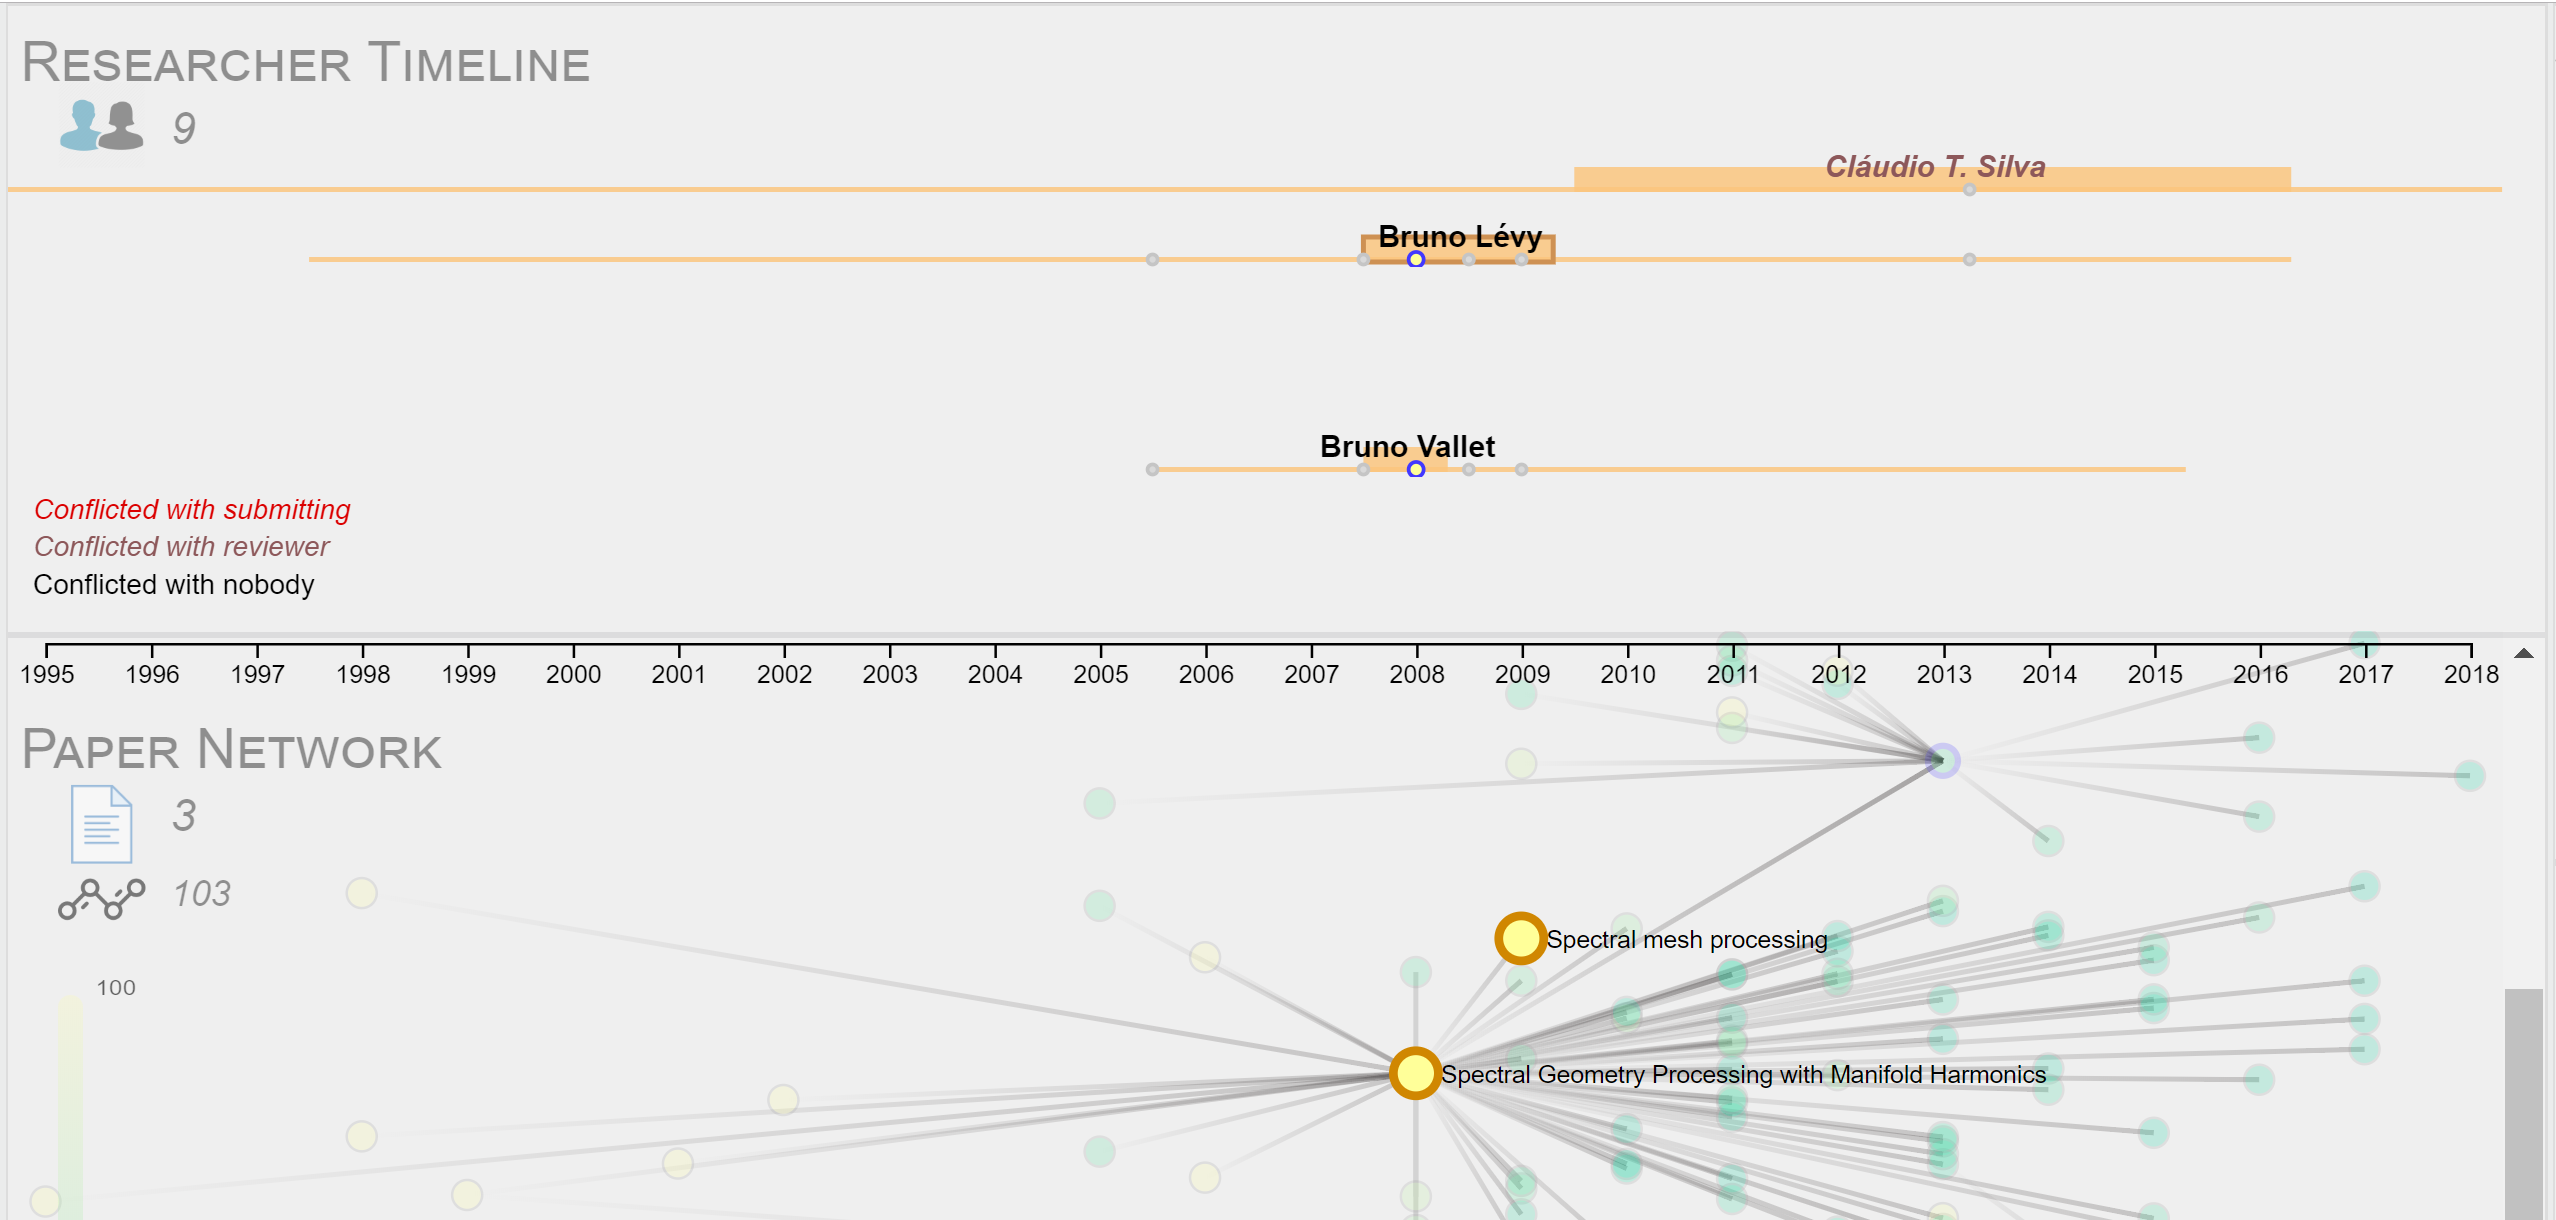
\includegraphics[width=\textwidth]{images/co-authors.png}
\caption{Focusing on a researcher by clicking on her/his name in the Researcher Timeline allows to highlight her/his co-authors and production in the Paper Network.}
\label{fig:co-authors}
\end{figure*}

\begin{figure*}
\centering
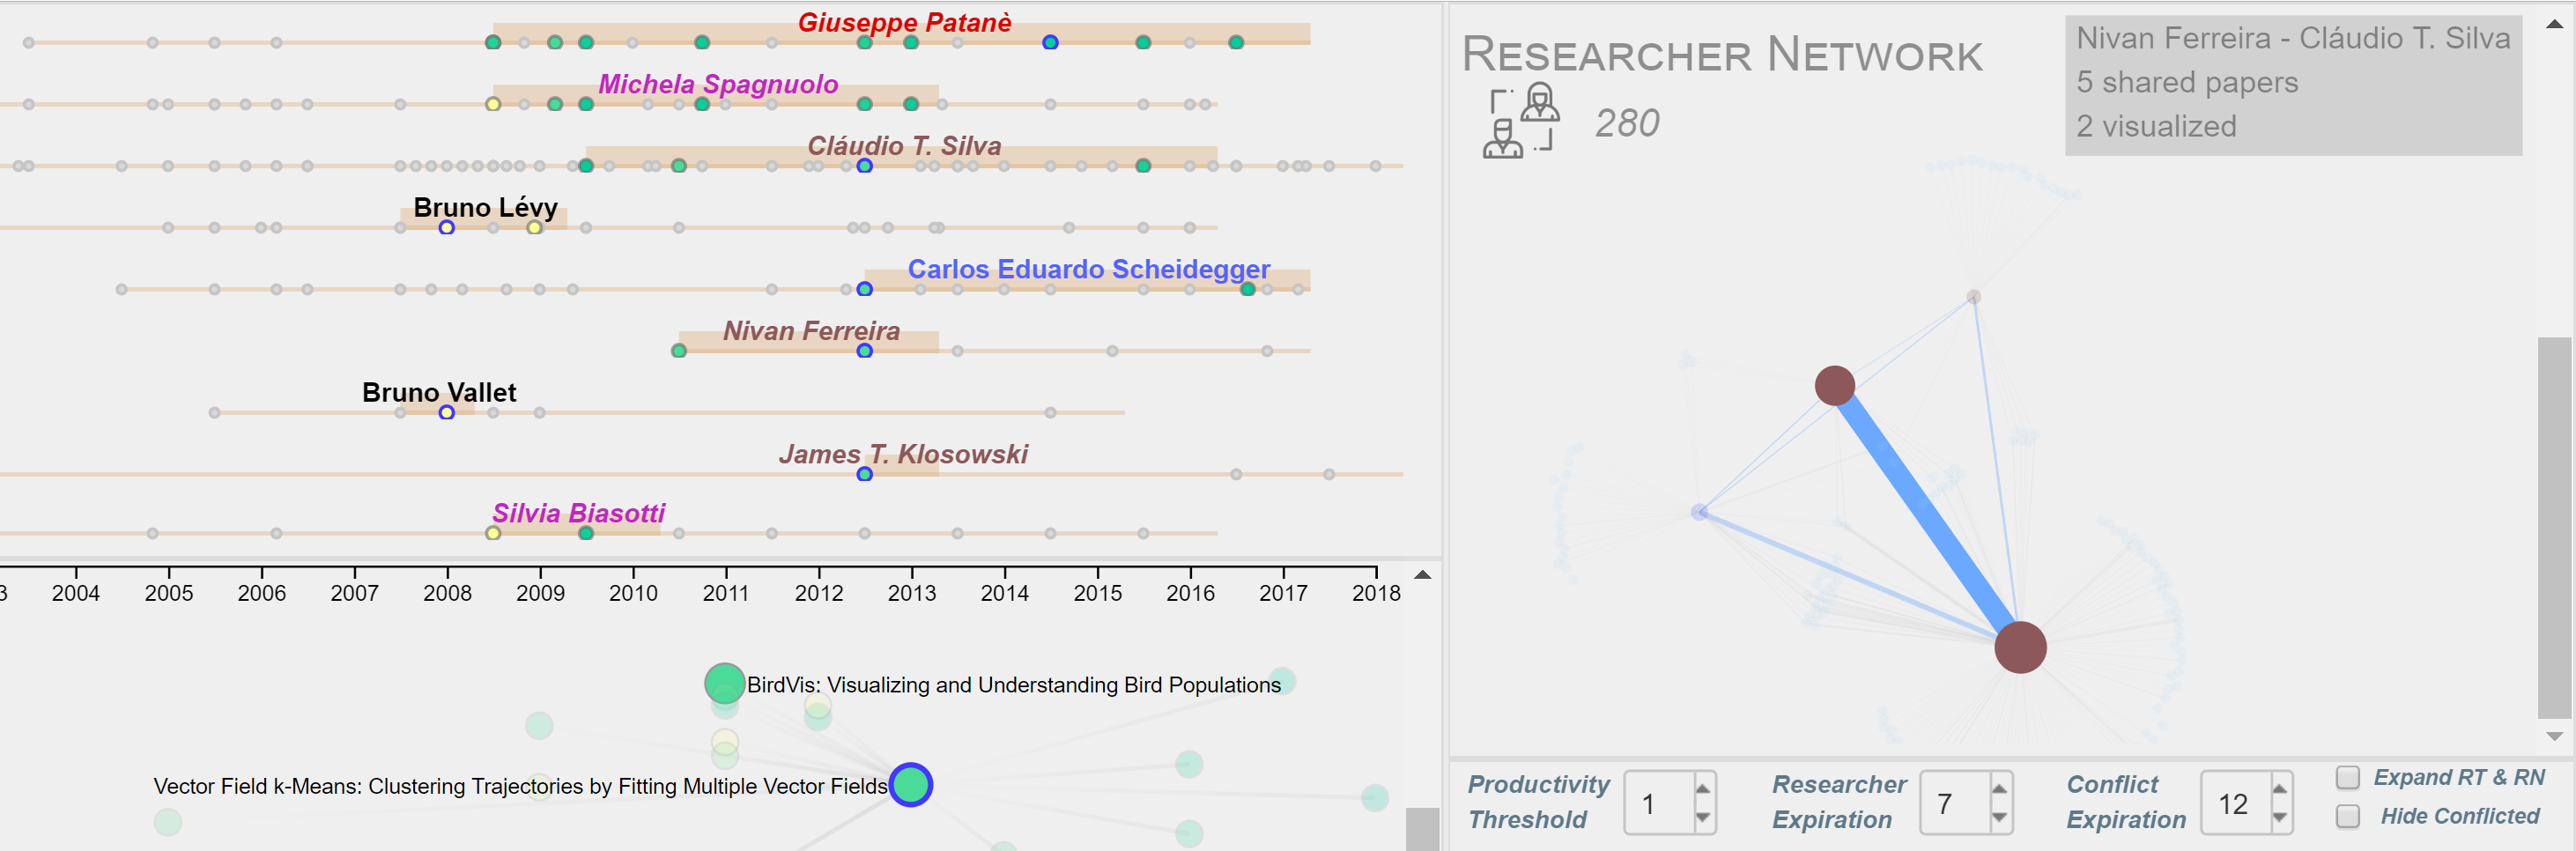
\includegraphics[width=\textwidth]{images/researchernetwork.png}
\caption{Hovering over a segment joining two researchers in the Researcher Network shows details about their co-authored papers and highlights them in the Paper Network.}
\label{fig:researchernetwork}
\end{figure*}

\begin{figure}
\centering
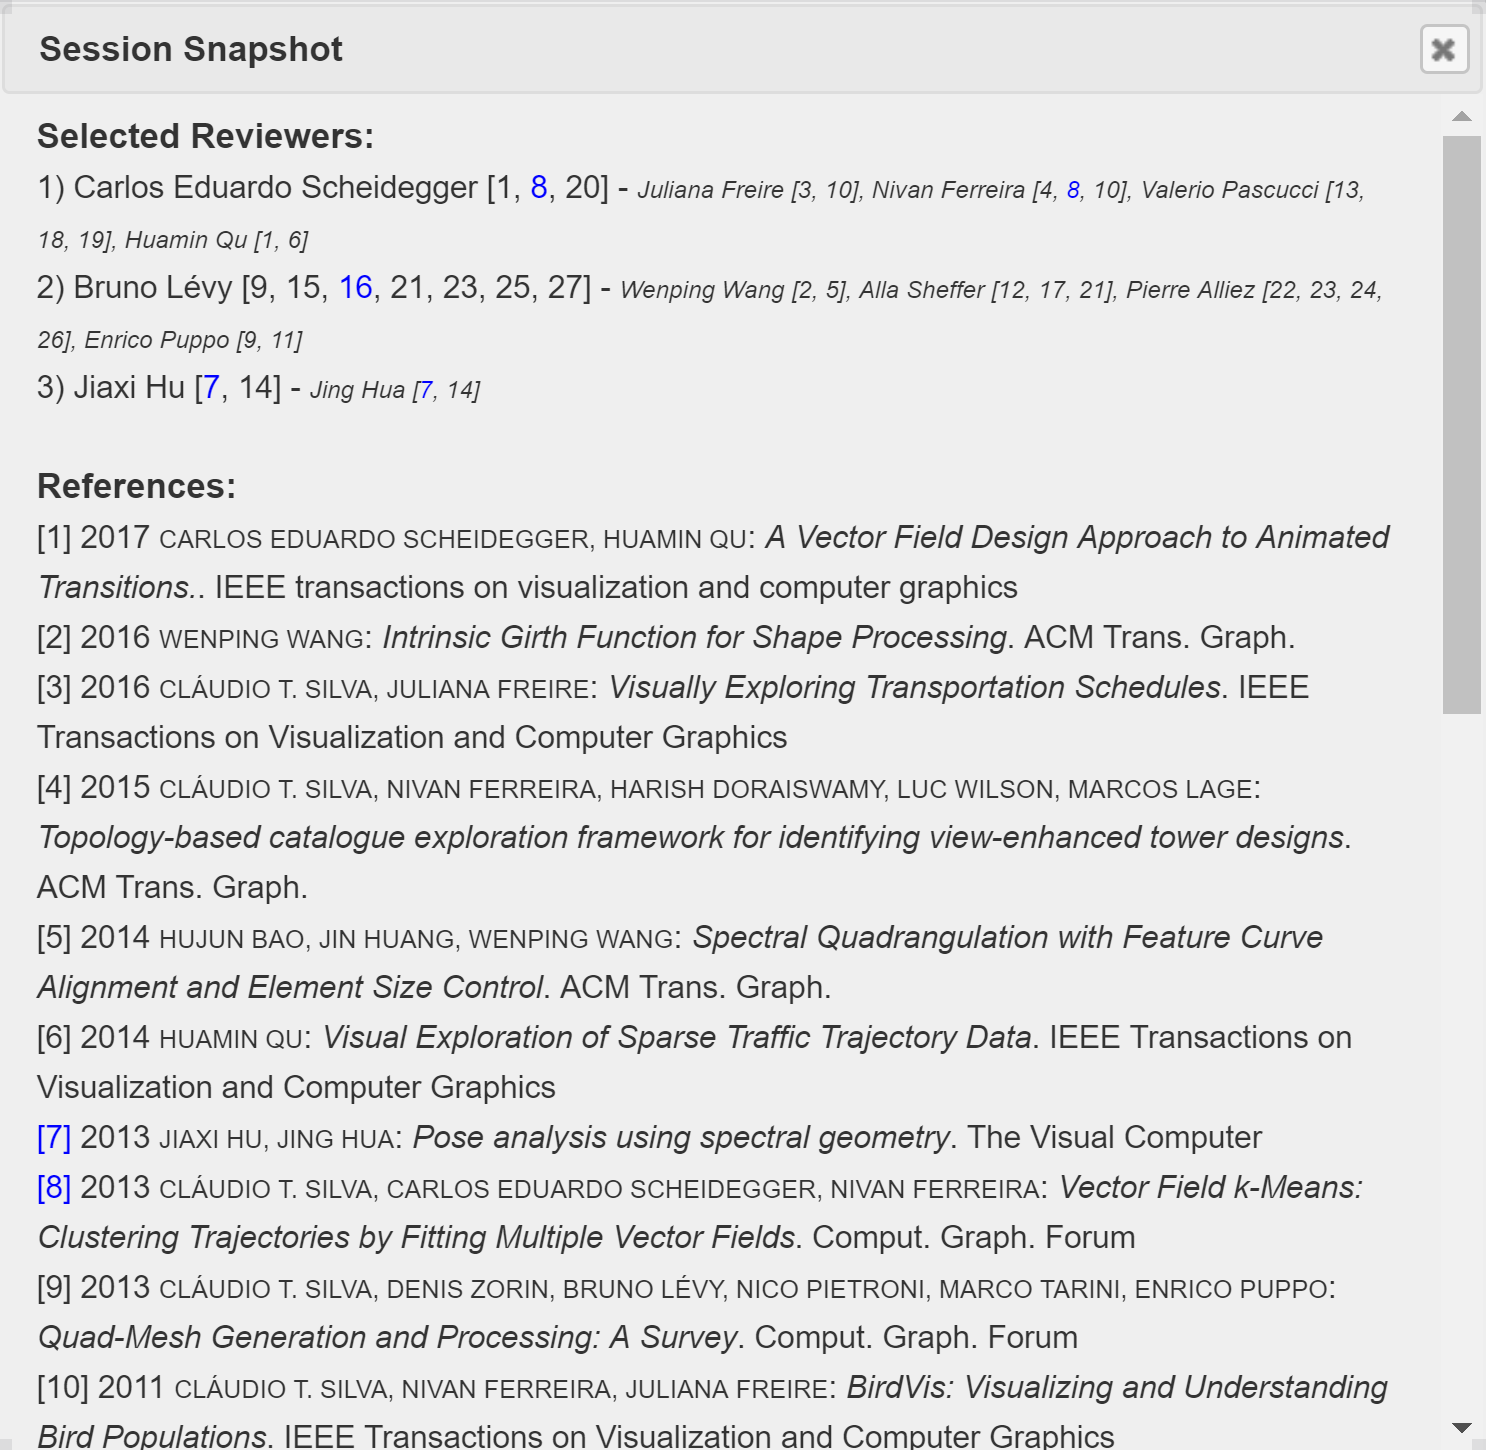
\includegraphics[width=0.7\textwidth]{images/list.png}
\caption{The list of selected reviewers together with substitutes and a bibliography. For each selected reviewer we list the papers he/she has authored and that motivated his/her choice as a reviewer.  The substitute reviewers are those researchers that have authored a similar set of publications and have the same conflicts as the selected reviewer, and therefore can replace him/her in case of decline.}
\label{fig:list}
\end{figure}


\section{Actions}
\label{subsec:actions}

Each view (PN, RT, RN, CP) is linked to the other views, so that any action in a view is reflected in the others. \\

\noindent{\bf Actions on Papers:} 
The first step is to build the Paper Network, that is, a set of key papers which are relevant to the submission topic. The user inizializes the PN by inputing the titles of a small set of seed papers in the \emph{Key papers} field, with the help of title-based suggestions. The seed papers are visualized in the PN, along with their in- and out-citations. The user can now expand the network, to discover additional documents. With a double click, he selects interesting nodes, i.e., papers he/she deems relevant to the submission topic. The PN then updates with the in- and out-citations of the selected papers. Papers can be deselected with a double click. 

When the users focuses on a paper in one of the views by mouse hovering, the same paper is highlighted in the other views. For example, when hovering the mouse over a node in the PN, the corresponding dot in the RT is highlighted, and viceversa. Also, the paper details (title, publication year, venue) are shown in the CP on a mouse click. Likewise, by hovering over or clicking on the title in the CP, the corresponding node and dot are highlighted in the PN and the RT.
       
When hovering the mouse over an entity representing a paper (a node in the PN, a dot in the RT bars, the title in the CP), the paper authors are highlighted in the RT and RN, if present (Figure \ref{fig:paperhovering}). A mouse click on the focused paper lets the user navigate the visualization with highlighted items. A single click restores the previous visualization.

The icon beside the paper title in the CP links to the DBLP page of the paper. \\

\noindent{\bf Actions on Researchers} In a similar fashion to papers, when the user focuses on a researcher in one of the views by mouse hovering, the same researcher is highlighted in the other views. When hovering the mouse over a node in the RN, the name of the corresponding researcher appears on the upper-right corner.  

When hovering the mouse over an entity representing a researcher (a bar in the RT, a dot in the RN, the name in the CP), the papers authored by the researcher are highlighted in the PN view. 

A mouse click on a researcher puts the focus on him/her, his/her production and his/her personal net of collaborators (Figure \ref{fig:co-authors}). The user can navigate a visualization with selected items and additional functionalities. Only the set of co-authors is visualized in the RT and the RN. While hovering on one of the co-authors, the common publications are shown in the PN, and the arc representing the co-authorship relation is visualized in the RN. Another mouse click will get the user back the previous visualization.

When hovering the mouse over an arc in the RT, a pop-up on the upper-right corner shows the pair of co-authors names, the number of common papers in the dataset $\mathcal{P}$, and the number of common relevant papers in $\mathcal{P}_{V}$. In turn, for blue arcs, the common papers are highlighted in the PN (Figure \ref{fig:researchernetwork}). 

The icon beside the researcher name in any of the fields in the CP links to the DBLP page of that researcher. 

A researcher can be removed from the list of selected reviewers with a double click.

Finally, for each reviewer selected by the user, ReviewerNet suggests a set of possible substitute reviewers, in case of negative answers from the selected one. For a selected reviewer $r$, the alternative reviewers are chosen in the set $\mathcal{R}_C$ of candidate reviewers, so that they only conflict with $r$, and with no other selected reviewer; the list of substitutes is ordered according to the number of common papers between the reviewer and his/her substitute. The user can exchange a reviewer with one of his/her substitutes by clicking on the name of the substitute.

Work sessions can be saved for later re-use and re-assessment.

The export button enables the user to download the list of reviewers and their potential substitutes. The list also includes references to the reviewers' publications in the dataset $\mathcal{P}$ (Figure \ref{fig:list}).  

\section{User-defined parameters and settings}
\label{subsec:parameters}

Users can adjust the number of candidate reviewers visualized through a set of thresholds and options. \\

\noindent{\bf Size of data visualized:} 
To limit the number of candidate reviewers visualized in the RT and the RN, the user can set two thresholds a researcher has to meet to be considered as a candidate reviewer: 
\begin{itemize}
\item \emph{Productivity threshold}: the minimum number of authored selected papers in $\mathcal{P}_S$ (i.e., $\vert \mathcal{P}_{S}|_{r} \vert$ has to be greater than the threshold, for a researcher $r$ to be included in the set $\mathcal{R}_C$ of candidate reviewers);
\item \emph{Researcher expiration}: the maximum number of years since the last authored paper in the reference dataset $\mathcal{P}$ (i.e., the number of years has to be lower than the threshold for a researcher to be considered active and included in $\mathcal{R}_C$).
\end{itemize}
The user can also remove conflicting authors and their co-authors from the visualization, by ticking the \emph{Hide Conflicted} checkbox.
To augment instead the number of potential reviewers visualized, the user can tick the \emph{Expand RT \& RN} checkbox: the visualization will include all the researchers in $\mathcal{R}_V$ (all the authors of relevant papers) instead of the researchers in $\mathcal{R}_C$ only (the authors of selected papers only). Note that visualizing a large number of researchers can slow down the interface. \\

\noindent{\bf Conflict-of-interest:} 
Finally, to modulate the conflict of interest, the user can set a threshold for two researchers to be considered as co-authors, namely 
\begin{itemize}
\item \emph{Conflict expiration}: the maximum number of years since the last co-authored paper in $\mathcal{P}$. 
\end{itemize}
A larger threshold will increase the number of candidates marked as conflicted. Conversely, a smaller threshold will increase the number of available reviewers. 


